

\let\negmedspace\undefined
\let\negthickspace\undefined
\documentclass[journal,12pt,twocolumn]{IEEEtran}
%\documentclass[conference]{IEEEtran}
%\IEEEoverridecommandlockouts
% The preceding line is only needed to identify funding in the first footnote. If that is unneeded, please comment it out.
\usepackage{svg}
\usepackage{tikz, pgfplots}
\usepackage{cite}
\usepackage{amsmath,amssymb,amsfonts,amsthm}
\usepackage{algorithmic}
\usepackage{float,graphicx}
\usepackage{textcomp}
\usepackage{xcolor}
\usepackage{txfonts}
\usepackage{listings}
\usepackage{enumitem}
\usepackage{mathtools}
\usepackage{gensymb}
\usepackage[breaklinks=true]{hyperref}
\usepackage{tkz-euclide} % loads  TikZ and tkz-base
\usepackage{listings}
\usetikzlibrary{positioning}
%
%\usepackage{setspace}
%\usepackage{gensymb}
%\doublespacing
%\singlespacing

%\usepackage{graphicx}
%\usepackage{amssymb}
%\usepackage{relsize}
%\usepackage[cmex10]{amsmath}
%\usepackage{amsthm}
%\interdisplaylinepenalty=2500
%\savesymbol{iint}
%\usepackage{txfonts}
%\restoresymbol{TXF}{iint}
%\usepackage{wasysym}
%\usepackage{amsthm}
%\usepackage{iithtlc}
%\usepackage{mathrsfs}
%\usepackage{txfonts}
%\usepackage{stfloats}
%\usepackage{bm}
%\usepackage{cite}
%\usepackage{cases}
\usepackage{subfig}
%\usepackage{xtab}
%\usepackage{longtable}
%\usepackage{multirow}
%\usepackage{algorithm}
%\usepackage{algpseudocode}
%\usepackage{enumitem}
%\usepackage{mathtools}
%\usepackage{tikz}
%\usepackage{circuitikz}
%\usepackage{verbatim}
%\usepackage{tfrupee}
%\usepackage{stmaryrd}
%\usetkzobj{all}
%    \usepackage{color}                                            %%
%    \usepackage{array}                                            %%
%    \usepackage{longtable}                                        %%
%    \usepackage{calc}                                             %%
%    \usepackage{multirow}                                         %%
%    \usepackage{hhline}                                           %%
%    \usepackage{ifthen}                                           %%
  %optionally (for landscape tables embedded in another document): %%
%    \usepackage{lscape}     
%\usepackage{multicol}
%\usepackage{chngcntr}
%\usepackage{enumerate}

%\usepackage{wasysym}
%\newcounter{MYtempeqncnt}
\DeclareMathOperator*{\Res}{Res}
%\renewcommand{\baselinestretch}{2}
\renewcommand\thesection{\arabic{section}}
\renewcommand\thesubsection{\thesection.\arabic{subsection}}
\renewcommand\thesubsubsection{\thesubsection.\arabic{subsubsection}}

\renewcommand\thesectiondis{\arabic{section}}
\renewcommand\thesubsectiondis{\thesectiondis.\arabic{subsection}}
\renewcommand\thesubsubsectiondis{\thesubsectiondis.\arabic{subsubsection}}

% correct bad hyphenation here
\hyphenation{op-tical net-works semi-conduc-tor}
\def\inputGnumericTable{}                                 %%

\lstset{
%language=C,
frame=single, 
breaklines=true,
columns=fullflexible
}
%\lstset{
%language=tex,
%frame=single, 
%breaklines=true
%}

\begin{document}
%


\newtheorem{theorem}{Theorem}[section]
\newtheorem{problem}{Problem}
\newtheorem{proposition}{Proposition}[section]
\newtheorem{lemma}{Lemma}[section]
\newtheorem{corollary}[theorem]{Corollary}
\newtheorem{example}{Example}[section]
\newtheorem{definition}[problem]{Definition}
%\newtheorem{thm}{Theorem}[section] 
%\newtheorem{defn}[thm]{Definition}
%\newtheorem{algorithm}{Algorithm}[section]
%\newtheorem{cor}{Corollary}
\newcommand{\BEQA}{\begin{eqnarray}}
		\newcommand{\EEQA}{\end{eqnarray}}
\newcommand{\define}{\stackrel{\triangle}{=}}

\bibliographystyle{IEEEtran}
%\bibliographystyle{ieeetr}


\providecommand{\mbf}{\mathbf}
\providecommand{\pr}[1]{\ensuremath{\Pr\left(#1\right)}}
\providecommand{\qfunc}[1]{\ensuremath{Q\left(#1\right)}}
\providecommand{\sbrak}[1]{\ensuremath{{}\left[#1\right]}}
\providecommand{\lsbrak}[1]{\ensuremath{{}\left[#1\right.}}
\providecommand{\rsbrak}[1]{\ensuremath{{}\left.#1\right]}}
\providecommand{\brak}[1]{\ensuremath{\left(#1\right)}}
\providecommand{\lbrak}[1]{\ensuremath{\left(#1\right.}}
\providecommand{\rbrak}[1]{\ensuremath{\left.#1\right)}}
\providecommand{\cbrak}[1]{\ensuremath{\left\{#1\right\}}}
\providecommand{\lcbrak}[1]{\ensuremath{\left\{#1\right.}}
\providecommand{\rcbrak}[1]{\ensuremath{\left.#1\right\}}}
\theoremstyle{remark}
\newtheorem{rem}{Remark}
\newcommand{\sgn}{\mathop{\mathrm{sgn}}}
\providecommand{\abs}[1]{\(left\)vert#1\(right\)vert}
\providecommand{\res}[1]{\Res\displaylimits_{#1}}
\providecommand{\norm}[1]{\(left\)lVert#1\(right\)rVert}
%\providecommand{\norm}[1]{\lVert#1\rVert}
\providecommand{\mtx}[1]{\mathbf{#1}}
\providecommand{\mean}[1]{E\(left\)[ #1 \(right\)]}
\providecommand{\fourier}{\overset{\mathcal{F}}{ \rightleftharpoons}}
%\providecommand{\hilbert}{\overset{\mathcal{H}}{ \rightleftharpoons}}
\providecommand{\system}{\overset{\mathcal{H}}{ \longleftrightarrow}}
%\newcommand{\solution}[2]{\textbf{Solution:}{#1}}
\newcommand{\solution}{\noindent \textbf{Solution: }}
\newcommand{\cosec}{\,\text{cosec}\,}
\providecommand{\dec}[2]{\ensuremath{\overset{#1}{\underset{#2}{\gtrless}}}}
\newcommand{\myvec}[1]{\ensuremath{\begin{pmatrix}#1\end{pmatrix}}}
\newcommand{\mydet}[1]{\ensuremath{\begin{vmatrix}#1\end{vmatrix}}}

\let\vec\mathbf


\vspace{3cm}

\title{
	%	\logo{
	Assignment:- 2
 
	\Large AI1110: Probability and Random Variables
 
	\Large Indian Institute of Technology, Hyderabad
	%	}
}
\author{
	CS22BTECH11001
	
	Aayush Adlakha
 
	29 April, 2023
	% <-this % stops a space
}






\maketitle

\newpage


\bigskip
\renewcommand{\thefigure}{\theenumi}
\renewcommand{\thetable}{\theenumi}
\textbf{12.13.5.12}
Find the probability of throwing at most 2 sixes in 6 throws of a single die.

\textbf{Solution.}
Let us define $X$ to be the number of times six appears on the dice,

Such that, 
\begin{align}
&\pr{X = i | X = i} = \frac{5}{6}\\
&\pr{X = i + 1 | X = i} = \frac{1}{6}
\end{align}
Therefore,
the process is a Markov process in which the $i$th state refers to six appearing $i$ times.

Transition Probabilities 
\begin{align}
    P_{i,i+1} &= \frac{1}{6}\\
    P_{i,i} &=\frac{5}{6}
\end{align}
For 6 throws,
\begin{figure}[h!]
    \centering
    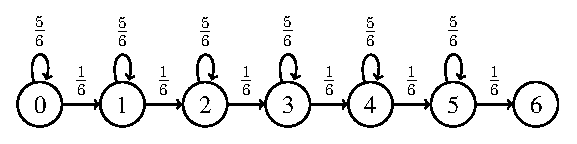
\includegraphics[width=\columnwidth]{figs/output-figure0}
    \caption{Transition Graph}
    \label{fig:my_label}
\end{figure}


The Transition Matrix of this chain is given by,
\begin{align}
A=\begin{bmatrix}
\frac{5}{6} & \frac{1}{6} & 0 & 0 & 0 & 0 & 0\\[6pt]
0 & \frac{5}{6} & \frac{1}{6} & 0 & 0 & 0 & 0\\[6pt]
0 & 0 & \frac{5}{6} & \frac{1}{6} & 0 & 0 & 0\\[6pt]
0 & 0 & 0 & \frac{5}{6} & \frac{1}{6} & 0 & 0\\[6pt]
0 & 0 & 0 & 0 & \frac{5}{6} & \frac{1}{6} & 0\\[6pt]
0 & 0 & 0 & 0 & 0 & \frac{5}{6} & \frac{1}{6}\\[6pt]
0 & 0 & 0 & 0 & 0 & 0 & \frac{5}{6}
\end{bmatrix}
\end{align}
This matrix represents the probabilities after one throw,

To calculate probabilities after 6 throws, we need to raise this matrix to the power 6

[This is analogous to adjacency matrix in Graph Theory]

On computation,
\begin{align}
  A^6 =   \begin{bmatrix}
  0.335 & 0.402 & 0.201 & 0.054 & 0.008 & 0.001 & 0.0 & \\
0 & 0.335 & 0.402 & 0.201 & 0.054 & 0.008 & 0.001 & \\
0 & 0 & 0.335 & 0.402 & 0.201 & 0.054 & 0.008 & \\
0 & 0 & 0 & 0.335 & 0.402 & 0.201 & 0.054 & \\
0 & 0 & 0 & 0 & 0.335 & 0.402 & 0.201 & \\
0 & 0 & 0 & 0 & 0 & 0.335 & 0.402 & \\
0 & 0 & 0 & 0 & 0 & 0 & 0.335 & \\
  \end{bmatrix}
\end{align}
Now, this is our transition matrix for 6 rolls of the dice.

Therefore, $P_{i,j}$ represents starting from $i$th state and ending up at $j$th state given 6 throws of dice.

For this question, we always start from $X=0$ and are required to end up with at-most 2 sixes or $X \le 2$.

\begin{align}
\label{eq:1}
    P_{0,0} &= 0.335\\
    \label{eq:2}
    P_{0,1} &= 0.402\\
    \label{eq:3}
    P_{0,2} &= 0.201
\end{align}
From \eqref{eq:1}, \eqref{eq:2} and \eqref{eq:3}
\begin{align}
    \pr{X \le 2} &= P_{0,0}+P_{0,1}+P_{0,2}\\
    &= 0.335+0.402+0.201\\
    &= 0.938
\end{align}
\end{document}